\newpage
\pagenumbering{arabic}  %numero de pagina numeración arábiga
\setcounter{page}{1}    %comienza a contar desde 1

\chapter{Introducción y objetivos}

%%% Dario: Esto va demasiado a los bifes, tenes que arrancar contando la importancia que tiene medir bien en fano.
%%% Lo que sigue es muy del plan presentado. Leete un par de introducciones de las tesis que tenes para enganchar con cual es la idea de esta introducción y lo charlamos.

\noindent Como parte de este trabajo se propuso el uso de técnicas de análisis de imágenes y procesamiento de datos propias de la física de partículas experimental. %, lo que llevó al fortalecimiento de conocimientos de estadística y la familiarización con el trabajo científico en un tema de creciente interés. 
Las metas propuestas en este trabajo son:
\begin{enumerate}
    \item Analizar las mediciones con luz LED para obtener una calibración absoluta de carga del detector a baja ocupancia y a diferentes temperaturas.
    \item Analizar las mediciones de rayos X producidos por desexcitación del flúor y aluminio, con el objetivo de determinar la energía de creación electrón hueco y el factor de Fano a $677\,\si{eV}$ y $1486\,\si{eV}$, respectivamente.
    \item Estudiar de la dependencia con la temperatura en el rango de $123$ a $160\,\si{K}$ de las cantidades anteriormente mencionadas.
    \item Estudiar la influencia de otras fuentes de fotones en la construcción de eventos y en la determinación del factor de Fano y energía de creación electrón hueco.
    \item Corregir el efecto que la luz espuria tiene sobre el valor medio de carga y su distribución.
\end{enumerate}

%%%%%%%%%%%%%%%%%%%%%%%%%%%%%%%%%%%%%%%%%%%%%%%%%%%%%%%%%%%%%%%%%%
%%%%%%%%%%%%%%%%%%%%%%%%%%%%%%%%%%%%%%%%%%%%%%%%%%%%%%%%%%%%%%%%%%
\section{Factor de Fano y energía de creación electrón-hueco}
\noindent El factor de Fano mide la dispersión de una distribución de carga producida en un detector y se define como
\begin{equation*}
    F = \frac{\sigma^{2}}{\mu}
\end{equation*}
donde $\sigma^{2}$ es la varianza de la distribución y $\mu$ es la media. 
Para el caso particular de una distribución de Poisson, la varianza y la esperanza coinciden, de forma que el factor de Fano equivale a $1$. Estas distribuciones de carga son el producto de la interacción de fotones de cierta energía con el detector, entre otros factores, que van depositando energía en el material ionizando cargas a su paso. El origen de dicha distribución radica en que la energía transferida en cada interacción no es constante y, por lo tanto, para una dada energía inicial de la partícula incidente, tampoco será constante el número de cargas generadas.\\
\indent Por otro lado, la energía de creación electrón-hueco $\varepsilon_{\eh}$ es, en valor medio, la energía necesaria para poder producir un par electrón-hueco en el interior del detector de Silicio. Así, esta puede ser calculada a través del cociente entre la energía entregada al detector y la carga producida en él. Además, ésta está relacionada con la energía del gap del silicio, entre la banda de valencia y la banda de conducción, que es $E_{g}\sim 1.1\,\si{eV}$\cite{Janesick}. Sin embargo, debido a que durante el proceso de interacción parte de la energía que entregada material puede disiparse emitiendo fonones, la energía de creación electrón-hueco resulta ser mayor, en promedio, que la energía del gap.\\
\indent La estimación precisa de ambas magnitudes es de vital importancia en la caracterización de este tipo de detectores, debido a que, por ejemplo, parámetros como la \textit{eficiencia cuántica} dependen fuertemente de ellos. Además es importante determinar la dependencia de estas magnitudes con la energía, ya que, en particular, el factor de Fano a energías por debajo de $1\,\si{keV}$ es clave para el cálculo de sensibilidad en experimentos de materia oscura liviana, como es caso del experimento SENSEI (\textit{Sub-Electron}
%%%%%%%%%%%%%%%%%%%%%%%%%%%%%%%%%%%%%%%%%%%%%%%%%%%%%%%%%%%%%%%%%%
%%%%%%%%%%%%%%%%%%%%%%%%%%%%%%%%%%%%%%%%%%%%%%%%%%%%%%%%%%%%%%%%%%
\section{CCD y Skipper CCD}
\noindent Los dispositivos CCD (\textit{Charge Coupled Devices}) fueron inventados en 1969 en los Laboratorios Bell, por Willard Boyle y George Smith, en su búsqueda por fabricar dispositivos de memoria. Finalmente, los CCD's no cumplieron este objetivo pero sí demostraron un gran potencial como sensores de luz y partículas. Tal es así que en el año 2010 sus inventores recibieron el premio Nobel de física\cite{Boyle}\cite{Smith}.\\
\indent Estos dispositivos están hechos esencialmente de Silicio y sus elementos constitutivos fundamentales son capacitores MOS (por \textit{metal-oxide-semiconductor}). Estos conforman los píxeles del detector, siendo por lo general millones y ocupando casi la totalidad de la superficie del sensor. Los capacitores MOS se componen generalmente de un sustrato semiconductor dopado, sobre el cual se deposita una delgada capa de óxido y a su vez sobre esta se coloca un metal de contacto. Este contacto metálico se encuentra a un voltaje $V_{G}$ y debajo del semiconductor se encuentra otro contacto que se encuentra a tierra. Dependiendo del valor de $V_{G}$ se obtienen distintos regímenes del MOS\footnote{citar} donde, en particular, uno de ellos genera una región de depleción cerca del óxido, el cual permite acumular carga minoritaria.\\

\indent El principio de operación de un CCD se puede dividir en cuatro etapas, que a grandes rasgos son:
\begin{itemize}
    \item Exposición del detector: El tiempo de exposición es variable y depende del tipo de medición que se desee utilizar. Durante la exposición, la radiación incidente interactúa con el detector, generalmente generando pares electrón-hueco. 
    \item Colección: Los electrones son luego arrastrados por el campo eléctrico del detector presente en su volumen hacia los pozos de potencial de los píxeles donde son colectados.
    \item Transferencia: Dado que la medición de los píxeles se realiza de forma secuencial, la carga en cada uno de ellos debe ser transferida de un píxel a otro.
    \item Medición de la carga: A medida que se desplaza la carga, esta es llevada hacia el nodo de sensado donde finalmente es medida.
\end{itemize}
Los CCD's convencionales son capaces de alcanzar ruidos de lectura del orden de los $2\,e^{-}\si{rms/pix}$, gracias a la técnica de muestreo doblemente correlacionado\cite{Tiffenberg}. Sin embargo, en aplicaciones de bajas energías, el ruido electrónico de lectura presupone una barrera al límite de energías que pueden medirse con estos sensores para mantener la precisión deseada.\\
\textcolor{red}{Figura de las mediciones del fano a baja energía}\\
\indent Los sensores \textit{Skipper}-CCD's, por otro lado, permiten disminuir el ruido electrónico de lectura a niveles subelectrónicos gracias a que son capaces de medir la carga en los píxeles de forma no destructiva. Esto permite tomar tantas mediciones como sean necesarias de la carga y estimar la carga real a partir de un promedio sobre el número de mediciones tomadas. El prácticamente ausente ruido de lectura que hace posible la capacidad de medir repetidas veces y de forma no destructiva la carga en cada píxel de un sensor \textit{Skipper}-CCD, tiene un fuerte impacto a energías por debajo de los $5\,\si{keV}$. En particular, por debajo de los $2\,\si{keV}$ la contribución del ruido de lectura de un CCD convencional a la determinación de estas cantidades puede superar el $30\,\%$. 
Esta es la principal razón que motiva este trabajo, donde se realiza un estudio sistemático del Factor de Fano a bajas energías, entre $1486\,\si{eV}$ (rayos X del Al) y $677\,\si{eV}$ (rayos X del F).\\


%%%%%%%%%%%%%%%%%%%%%%%%%%%%%%%%%%%%%%%%%%%%%%%%%%%%%%%%%%%%%%%%%%
%%%%%%%%%%%%%%%%%%%%%%%%%%%%%%%%%%%%%%%%%%%%%%%%%%%%%%%%%%%%%%%%%%
\section{Antecedentes}

\noindent En trabajos previos se han estudiado las ventajas de la utilización de la novedosa tecnología \textit{Skipper}-CCD, para lograr medir con precisión subelectrónica en regímenes de energía donde los sensores CCD convencionales más precisos sólo podrían alcanzar resoluciones del orden de los $2$ electrones. Por primera vez fue usada para poder medir el factor de Fano y la energía de creación electrón-hueco en el Silicio a una energía de $5.9\,\si{keV}$ a $123\,\si{K}$\cite{Rodrigues}.\\
\indent Para lograr esto, se implementó un método de calibración absoluta que determinó la relación entre el número de electrones en cada píxel y la lectura del valor en ADUs (\textit{Analog Digital Unit} o Unidades analógico-digitales). El procedimiento para la calibración consistió en la utilización de un LED instalado en el \textit{dewar}, que emitía fotones en $405\,\si{nm}$ de longitud de onda, para poblar los píxeles del sensor. Así, lograron poblar los píxeles en un amplio rango de cargas realizando un barrido en el tiempo de exposición del sensor a la luz LED. Las mediciones posteriores de la carga por píxel se realizaron tomando $300$ lecturas de cada píxel, gracias a la tecnología \textit{Skipper} que permite realizar estas lecturas de forma no destructiva, y que luego fueron promediadas, se logra reducir el ruido de lectura en un factor $\sqrt{300}$. Como resultado de estas mediciones, se generaron distribuciones de carga Gaussianas en los posibles niveles de ocupación de carga, superpuestas entre sí y desfasadas en valor medio con excelente resolución, haciendo posible distinguir entre picos consecutivos. De esta forma, mediante un ajuste gaussiano se pudo establecer el valor medio en ADUs para cada uno de estos picos, estableciendo como valor de carga el número de pico correspondiente. Así es que se obtuvo una relación $1$ a $1$ entre cantidad de carga por píxel y ADUs. Cabe destacar que para comenzar a numerar los picos, primero es necesario establecer el valor de $0$ carga, es decir, píxel vacío, lo cual no corresponde a un valor nulo en ADUs.\\
Para ello, las imágenes tomadas con Skipper cuentan con una región denominada \textit{overscan} que se utiliza para calcular la linea de base y poder substraerla luego a la carga de cada píxel, logrando así que la media de los pixeles vacíos quede en cero ADUs.

\indent Por otro lado, por primera vez se midieron el factor de Fano $F$ de forma absoluta y la energía de creación electrón-hueco $\varepsilon_{\eh}$ utilizando esta tecnología. Esto se realizó midiendo rayos $X$ de $5.9\,\si{\mbox{keV}}$ emitidos por una fuente de $\prescript{55}{}{\mbox{Fe}}$. Más precisamente, rayos $X_{K}$, cuyas energías son los de la tabla \ref{tab:EnergiasXk}.
\begin{table}[h]
\centering
\begin{tabular}{@{}ccc@{}}
\toprule
$X_{K}$         &   Energía [keV]   &   Intensidad relativa \\ \hline \hline
$\alpha_{2}$    &   $5887.6$        &   $8.5 (4)$           \\
$\alpha_{1}$    &   $5898.8$        &   $16.9 (8)$          \\
$\beta_{3}$     &   $6490.4$        &   $4.1 (11)$          \\ \bottomrule
\end{tabular}
\caption{\footnotesize{Energías e intensidades relativas de los fotones X emitidos tras el decaimiento de $\prescript{55}{}{\mbox{Fe}}$}}
\label{tab:EnergiasXk}
\end{table}
Sobre los resultados de las mediciones realizadas para estos rayos $X$, se realizó un ajuste no bineado de los picos del espectro. Para realizar el ajuste se utilizó la verosimilitud, cuya expresión es la de la ecuación \eqref{ec:verosimilitud}, que surge de la convolución de dos distribuciones exponenciales y una distribución gaussiana
{\small
\begin{align}
    \Lagr(e|\mu_{1},
            \mu_{2},
            \sigma_{1},
            \lambda_{1},
            \lambda_{2},
            \eta_{1} = \eta_{2},
            \eta_{3})
    = &
    \sum\limits_{j=1}^{3} I_{j}
    \left\{
        \eta_{j}\frac{\lambda_{1}}{2}
        \exp
            \left[
                (e-\mu_{j})\lambda_{1} + \frac{\sigma_{j}^{2}\lambda_{1}^{2}}{2}
            \right]
        \mbox{Erfc}
        \left[
            \frac{1}{\sqrt{2}}
            \left(
                \frac{e - \mu_{j}}{\sigma_{j}}
                +\sigma_{j}\lambda_{1}
            \right)
        \right] \right. \nonumber
        \\
        + &
        \left.
        (1-\eta_{j})\frac{\lambda_{2}}{2}
        \exp
            \left[
                 (e - \mu_{j})\lambda_{2}
                 + \frac{\sigma_{j}^{2}\lambda_{2}^{2}}{2}
            \right]
        \mbox{Erfc}
        \left[
            \frac{1}{\sqrt{2}}
            \left(
                \frac{e - \mu_{j}}{\sigma_{j}}
                +\sigma_{j}\lambda_{2}
            \right)
        \right]
    \right\}
        \label{ec:verosimilitud}
\end{align}
}
donde $\mu_{j}$, $\sigma_{j}$ y $I_{j}$ representan el valor medio de carga, la desviación estándar del valor medio de carga y la intensidad relativa del pico $j$-ésimo con energía $E_{j}$, respectivamente. Además, $\lambda_{1}$ y $\lambda_{2}$ son parámetros de la distribuciones exponenciales y $\eta_{j}$ es el peso relativo entre ellas.\\
\indent La figura \ref{fig:AjusteNoBineado} representa el ajuste no bineado por la verosimilitud de los picos de rayos $X$ para un total de $18085$ eventos. Lo resultados para la medición del factor de Fano, la energía de creación electrón-hueco y demás parámetros relevantes se encuentran en la tabla \ref{tab:ParametrosAjusteNoBineado}.
\begin{figure}%[H]
    \centering
        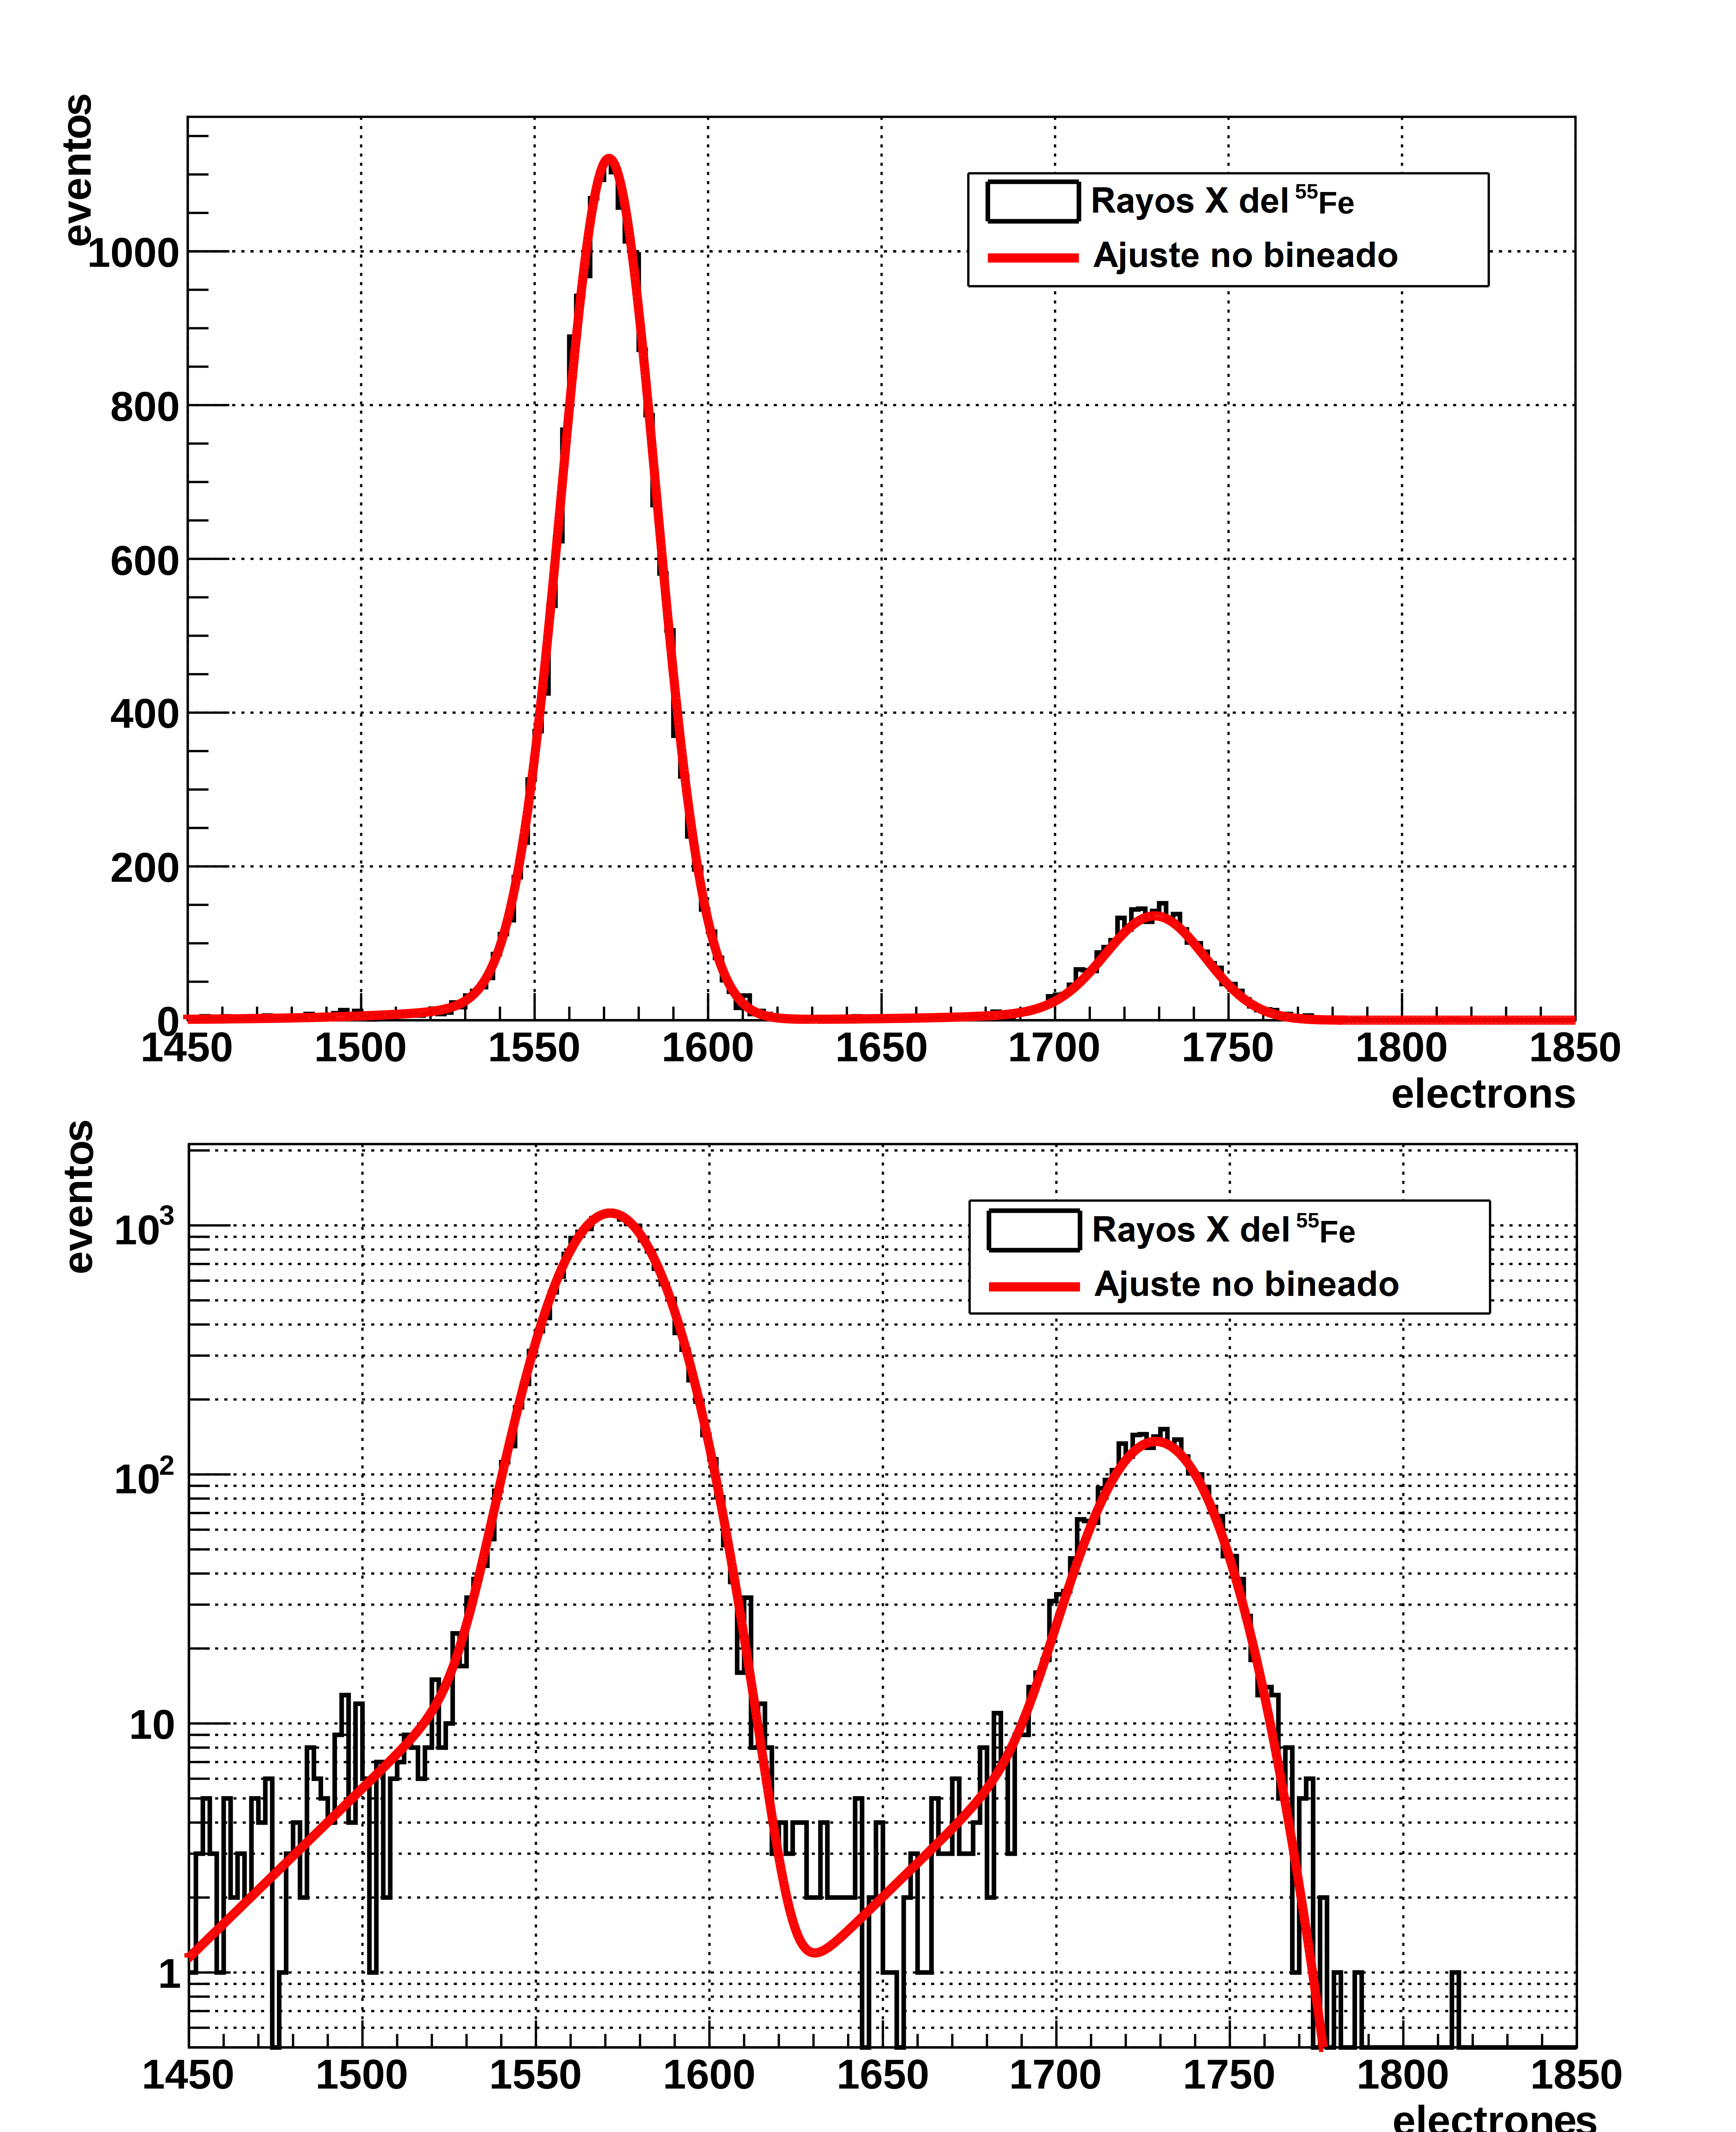
\includegraphics[scale=.15]{Figs/AjusteNoBineado.png}
    \caption{\footnotesize{Ajuste no bineado de los picos de $\prescript{55}{}{\mbox{Fe}}$.}}
    \label{fig:AjusteNoBineado}
\end{figure}
\begin{table}[h]
\centering
\begin{tabular*}{\textwidth}{c @{\extracolsep{\fill}} ccccccccc}%{@{}ccccccccc@{}}
\toprule
$X_{K}$ &
  $\mu\ [e^{-}]$ &
  $\Delta \mu\ [e^{-}]$ &
  $\sigma\ [e^{-}]$ &
  $\Delta \sigma\ [e^{-}]$ &
  $F$ &
  $\Delta F$ &
  $\varepsilon_{\eh}\ [\mbox{eV}/e^{-}]$ &
  $\Delta \varepsilon_{\eh} \ [\mbox{eV}/e^{-}]$ \\ \hline\hline
$\alpha_{2}$ &
  $1570.50$ &
  $0.18$ &
  $13.68$ &
  $0.12$ &
  \multirow{3}{*}{$0.119$} &
  \multirow{3}{*}{$0.002$} &
  \multirow{2}{*}{$3.749$} &
  \multirow{2}{*}{$0.001$} \\
$\alpha_{1}$ & $1573.48$ & $0.18$ & $13.69$ & $0.12$ &  &  &         &         \\
$\beta_{3}$  & $1730.50$ & $0.55$ & $14.36$ & $0.13$ &  &  & $3.751$ & $0.002$ \\ \bottomrule
\end{tabular*}
\caption{tabla}
\label{tab:ParametrosAjusteNoBineado}
\end{table}
Estos constituyen los primeros resultados obtenidos de la utilización de la tecnología \textit{Skipper}-CCD para el cálculo del factor de Fano y de la energía de creación electrón-hueco para una temperatura de $123\,\si{K}$ y se encontraron en buen acuerdo con la bibliografía preexistente~\cite{Ryan, Alig, Kotov}.\\
%Comentarios
\indent Además, se avanzó en las primeras mediciones del factor de Fano y la energía de creación electrón-hueco para energías por debajo de los de $2\,\si{keV}$~\cite{TesisKevin}, más específicamente, para energías de $677\,\si{eV}$ y $1486\,\si{eV}$, que corresponden a los rayos $X$ de fluorescencia del Flúor y del Aluminio respectivamente. En la tabla \ref{tab:EnergiasFluorescenciaFAl} pueden verse las energías e intensidades relativas para los rayos $X$ de estos elementos. En este caso, utilizando toda la maquinaria desarrollada en el trabajo anterior, realizaron mediciones con una fuente de $\prescript{241}{}{\mbox{Am}}$ que emite partículas alfa con una energía de $\sim 5.6\,\si{MeV}$. A estas partículas luego se las hizo impactar contra una cinta de teflón y una barra de aluminio que por fluorescencia emitían rayos $X$ con las energías antes mencionadas. Cabe destacar que se trató de evitar que las partículas alfa alcanzaran el detector, dado que son partículas muy energéticas y por tanto no son eventos de interés.\\
\indent Uno de los desafíos que surgieron en este otro trabajo fue que solo una fracción de los átomos que son impactados por las partículas alfa se desexcitan emitiendo fotones $X$ en las energías de interés. Es por esto que la tasa de eventos medidos es considerablemente menor en comparación a la que se obtuvo al medir con la fuente de $\prescript{55}{}{\mbox{Fe}}$.
\begin{table}[h]
\centering
\begin{tabular}{@{}cccc@{}}
\toprule
Elemento    &   $X_{K}$         &   Energía [eV]    &   Intensidad relativa \\ \hline \hline
F           &   $\alpha_{1,2}$  &   $676.8$         &   $148$               \\
Al          &   $\alpha_{2}$    &   $1486.3$        &   $50$                \\
Al          &   $\alpha_{1}$    &   $1486.7$        &   $100$               \\
Al          &   $\beta_{1}$     &   $1557.4$        &   $1$                 \\ \bottomrule
\end{tabular}
\caption{\footnotesize{Caption}}
\label{tab:EnergiasFluorescenciaFAl}
\end{table}
Con los datos de estas mediciones se reconstruyeron los espectros para ambos picos y se les realizó un ajuste no bineado, similar al utilizado en los experimentos con $\prescript{55}{}{\mbox{Fe}}$, utilizando la verosimilitud descripta por la expresión \eqref{ec:verosimilitudF-Al}.
\begin{align}
    \Lagr(e|\mu,
            \sigma,
            \lambda_{1},
            \lambda_{2},
            \eta)
    = &
    \eta
    \left\{
        \frac{\lambda_{1}}{2}
        \exp\left[
                (e-\mu)\lambda_{1} + \frac{\sigma^{2}\lambda_{1}^{2}}{2}
            \right]
        \mbox{Erfc}
        \left[
            \frac{1}{\sqrt{2}}
            \left(
                \frac{e - \mu}{\sigma}
                +\sigma\lambda_{1}
            \right)
        \right] \right\} \nonumber
        \\
        + &
        (1-\eta)
        \left\{
        \frac{\lambda_{2}}{2}
        \exp
            \left[
                 (e - \mu)\lambda_{2}
                 + \frac{\sigma^{2}\lambda_{2}^{2}}{2}
            \right]
        \mbox{Erfc}
        \left[
            \frac{1}{\sqrt{2}}
            \left(
                \frac{e - \mu}{\sigma}
                +\sigma\lambda_{2}
            \right)
        \right]
    \right\}
        \label{ec:verosimilitudF-Al}
\end{align}
En este caso, el ajuste no bineado resultó mucho más sensible a los cambios en el bineado del histograma, debido a que la tasa de eventos registrados para este experimento fue mucho menor. Los resultados obtenidos en este trabajo a partir de los ajustes de estas mediciones se encuentran en la tabla \ref{tab:ParametrosAjusteNoBineadoF-Al}.\\
\begin{table}[h]
\centering
\begin{tabular*}{\textwidth}{c @{\extracolsep{\fill}} ccccccccc}%{@{}ccccccccc@{}}
\toprule
Elemento&
  $\mu\ [e^{-}]$ &
  $\Delta \mu\ [e^{-}]$ &
  $\sigma\ [e^{-}]$ &
  $\Delta \sigma\ [e^{-}]$ &
  $F$ &
  $\Delta F$ &
  $\varepsilon_{\eh}\ [\mbox{eV}/e^{-}]$ &
  $\Delta \varepsilon_{\eh} \ [\mbox{eV}/e^{-}]$ \\ \hline\hline
  F &   $182.0$ &   $0.8$  &   $7.0$   &   $0.7$   &   $0.27$  &   $0.05$  &   $3.72$ &   $0.02$\\
  Al&   $404.4$ &   $0.4$  &   $8.3$   &   $0.3$   &   $0.17$  &   $0.01$  &   $3.679$ &   $0.004$\\ \bottomrule
\end{tabular*}
\caption{tabla}
\label{tab:ParametrosAjusteNoBineadoF-Al}
\end{table}
\indent Hasta aquí los resultados previos obtenidos con la utilización de esta novedosa tecnología de \textit{Skipper}-CCD para la medición del factor de Fano y la energía de creación electrón hueco. Sin embargo, todavía se pueden mejorar los resultados aumentando la estadística de los eventos para las energías inferiores a $2\,\si{keV}$ caracterizando el fondo presente en las imágenes. Para lograr esto es necesario realizar un tratamiento sobre los datos existentes.
%%%%%%%%%%%%%%%%%%%%%%%%%%%%%%%%%%%%%%%%%%%%%%%%%%%%%%%%%%%%%%%%%%
%%%%%%%%%%%%%%%%%%%%%%%%%%%%%%%%%%%%%%%%%%%%%%%%%%%%%%%%%%%%%%%%%%
\section{Motivación del análisis de imágenes}
\noindent Este trabajo se centró en la determinación del factor de Fano y de la energía de creación electrón-hueco, para energías por debajo de los $2\,\si{keV}$, utilizando mediciones preexistentes. Más precisamente, para las energías de los rayos $X$ de fluorescencia del Aluminio de $1486\,\si{eV}$ y del Flúor de $677\,\si{eV}$. Con el fin de que la determinación de estas características esté lo menos sesgada posible debido al fondo presente en las imágenes, fue necesario realizar un análisis profundo de los datos.\\
\indent El fondo presente en las imágenes consiste principalmente en píxeles cuya carga es producida por fluctuaciones térmicas en la red cristalina del Silicio del sensor (corrientes oscuras), por eventos de dispersión producidos por rebotes dentro del dispositivo de medición y que no deseados, y por eventos muy penetrantes provenientes del exterior, como por ejemplo, muones.\\
\indent El análisis consistió en estudiar el efecto que produce el fondo de las imágenes sobre los eventos de interés: la aglomeración de píxeles con cargas entre $1$ y $2$ electrones alrededor de los clusters, y la carga extra añadida sobre ellos. En muchos casos resulta que los píxeles con fondo se aglutinan a los clusters, aumentando su tamaño y su carga, o incluso también haciendo de puente entre dos clusters vecinos. Estos son dos efectos indeseados, primero porque sesga la cantidad de carga real en un evento de interés y segundo porque los algoritmos de clusterizacion podrían ignorarlos al no cumplir con los cortes de calidad impuestos, tanto por forma como por cantidad de carga esperada.\\
\indent Es entonces necesario utilizar un umbral de detección que ignore estos píxeles con carga menor o igual a $2$ electrones, de forma de evitar el aglutinamiento de píxeles con fondo a los clusters de interés y así aumentar la estadística en el conteo de eventos. Pero también es necesario lograr caracterizar este fondo para corregir el sesgo introducido por el nuevo umbral de detección, el cual, también eliminará píxeles con carga genuina. Es por eso que en este trabajo se propuso un análisis de las imágenes para poder determinar el umbral más conveniente a utilizar y recuperar la mayor cantidad de estadística posible, además de un método para estimar cuántos eventos genuinos son removidos y cuántos eventos espurios hay que remover de los clusters para mejorar así las incertezas del factor de Fano y la energía de creación electrón-hueco a bajas energías.
%%%%%%%%%%%%%%%%%%%%%%%%%%%%%%%%%%%%%%%%%%%%%%%%%%%%%%%%%%%%%%%%%%
%%%%%%%%%%%%%%%%%%%%%%%%%%%%%%%%%%%%%%%%%%%%%%%%%%%%%%%%%%%%%%%%%%
\section{Organización de la tesis}
Esto lo escribo al final y es un resumen de como está armada la tesis.
%%%%%%%%%%%%%%%%%%%%%%%%%%%%%%%%%%%%%%%%%%%%%%%%%%%%%%%%%%%%%%%%%%
%%%%%%%%%%%%%%%%%%%%%%%%%%%%%%%%%%%%%%%%%%%%%%%%%%%%%%%%%%%%%%%%%%
%%%%%%%%%%%%%%%%%%%%%%%%%%%%%%%%%%%%%%%%%%%%%%%%%%%%%%%%%%%%%%%%%%